\documentclass[10pt,a4paper,twoside,american]{article}
\usepackage{geometry}
\geometry{verbose,a4paper,tmargin=2cm,bmargin=2cm,lmargin=2cm,rmargin=2cm}
\usepackage{authblk}
\usepackage{calc}
\usepackage{graphicx}
\usepackage[table]{xcolor}
\definecolor{shadecolor}{gray}{0.9}
\usepackage{natbib} 
\usepackage[font=small,labelfont=bf]{caption}
\usepackage{amsmath}
\usepackage{amssymb}
\usepackage{mathtools}
\usepackage{bm}
\usepackage{algorithmic}

\usepackage[%%
breaklinks=true,
colorlinks=true,
linkcolor=gray,citecolor=gray,urlcolor=gray,filecolor=gray,
pdffitwindow,
bookmarks=true,
bookmarksopen=true,
bookmarksnumbered=true,
pdftitle={},
pdfauthor={},
pdfsubject={},
pdfkeywords={}
]
{hyperref}
%%%%%%%%%%%%%%%%%%%%%%%%%%%%%
%%%% change tracking
\usepackage{changes} %% see documentation @ https://ctan.org/pkg/changes
%% define authors and their colors
\definecolor{YB}{RGB}{0,0,200}
\definecolor{TT}{RGB}{0,200,0}
\definecolor{DW}{RGB}{200,0,0}
\definechangesauthor[color=YB]{YB}
\definechangesauthor[color=TT]{TT}
\definechangesauthor[color=DW]{DW}

\newcommand{\note}[2][]{\added[#1]{\footnotesize\it[#2]}} %% add \note command for notes
%%%%%%%%%%%%%%%%%%%%%%%%%%%%%
%%%% crosslinks
\usepackage{cleveref}
\crefformat{equation}{(#1)}
\crefformat{figure}{Fig.\,#1}
\crefformat{section}{Sec.\,#1}
\crefformat{table}{Tab.\,#1}

\usepackage[]{float}
\restylefloat{figure}
%%%%%%%%%%%%%%%%%%%%%%%%%%%%%
%% NEURON specific formating (see author guidelines: https://www.cell.com/neuron/authors)
\renewcommand\familydefault{cmss}      %% NEURON is using sans-serif fonts
\renewcommand{\abstractname}{Summary}  %% abstract is called Summary 

\def\figdir{figures}

%% macros
\newcommand{\panel}[3]{%         
  \parbox[t]{2ex}{\textbf{#1}\,}
  \parbox[t]{#2}{\,\includegraphics[width=#2]{#3}}
}

\newcommand{\seq}[1]{\ensuremath{\{\text{#1}\}}}



%%%%%%%%%%%%%%%%%%%%%%%%%%%%%%%%%%%
%% sorted alphabetically
\newcommand{\CM}{C_\textnormal{m}}    %% membrane time constant
\newcommand{\CV}{\textnormal{CV}}     %% coefficient of variation
\newcommand{\dtfilter}{\Delta t_\textnormal{f}}
\newcommand{\dtpert}{\delta t^*}
\newcommand{\dtsim}{\Delta t}
\newcommand{\DS}{\textnormal{DS}}
\newcommand{\EE}{{\exc\exc}}
\newcommand{\EI}{{\exc\inh}}
\newcommand{\EF}{{\exc\textnormal{F}}}
\newcommand{\exc}{\textnormal{E}}     %% label for ``excitatory''
\newcommand{\ext}{\textnormal{X}}   %% label for ``external''
\renewcommand{\exp}{\textnormal{exp}} %% exponential function
\newcommand{\erf}{\textnormal{erf}} %% error function
\newcommand{\EW}[2][]{\left\langle{#2}\right\rangle_{#1}}
\newcommand{\FF}{\textnormal{FF}}     %% Fano factor
\newcommand{\IE}{{\inh\exc}}
\newcommand{\II}{{\inh\inh}}
\newcommand{\EX}{{\exc\ext}}
\newcommand{\Epop}{\mathcal{E}} %% set (hence caligraphic) of excitatory neurons
\newcommand{\inh}{\textnormal{I}}     %% label for ``inhibitory''
\newcommand{\Ipop}{\mathcal{I}} %% set (hence caligraphic) of inhibitory neurons
\newcommand{\Imag}{\textnormal{Im}}
\newcommand{\PSCamp}{\hat{I}}               %% PSC amplitude (pA)
\newcommand{\J}{J}                          %% PSP amplitude (mV)
\newcommand{\JE}{{\J_{\exc}}}
\newcommand{\JEE}{\J_{\exc\exc}}
\newcommand{\JEI}{\J_{\exc\inh}}
\newcommand{\JI}{\J_{\inh}}
\newcommand{\JIE}{\J_{\inh\exc}}
\newcommand{\JII}{\J_{\inh\inh}}
\newcommand{\JEX}{\J_{\exc\ext}}
\newcommand{\JX}{\J_\ext}
\newcommand{\K}{K}
\newcommand{\KD}{K_{\textnormal{D}}}
\newcommand{\KE}{K_{\exc}}
\newcommand{\KEE}{{K_{\exc\exc}}}
\newcommand{\KEI}{{K_{\exc\inh}}}
\newcommand{\KI}{{K_{\inh}}}
\newcommand{\KIE}{{K_{\inh\exc}}}
\newcommand{\KII}{{K_{\inh\inh}}}
\newcommand{\Kinput}{{K^\textnormal{out}_\ext}} %% outdegree of each inpu sources
\newcommand{\KX}{{K_\ext}} %% number of inputs from external sources (external in-degree)
\newcommand{\mat}[1]{\bm{#1}}
\renewcommand{\max}{\textnormal{max}} %% exponential function
\newcommand{\ms}{\,\textnormal{ms}}
\newcommand{\muE}{{\mu_\exc}}
\newcommand{\muI}{{\mu_\inh}}
\newcommand{\mV}{\,\textnormal{mV}}
\newcommand{\ND}{{N_{\textnormal{D}}}}
\newcommand{\NE}{{N_{\exc}}}
\newcommand{\NI}{{N_{\inh}}}
\newcommand{\nE}{{n_\exc}}
\newcommand{\nI}{{n_\inh}}
\newcommand{\pA}{\,\textnormal{pA}}
\newcommand{\pert}{\textnormal{pert}}
\newcommand{\pF}{\,\textnormal{pF}}
\newcommand{\Real}{\textnormal{Re}}
\newcommand{\RM}{R_\textnormal{m}}
\newcommand{\s}{\,\textnormal{s}}
\newcommand{\seconds}{\,\textnormal{s}}
\newcommand{\sigmaE}{\sigma_{\exc}}
\newcommand{\sigmaI}{\sigma_{\inh}}
\newcommand{\sps}{\,\textnormal{spikes/s}}
\newcommand{\syn}{\textnormal{s}}
\newcommand{\tauM}{\tau_\textnormal{m}}
\newcommand{\tauR}{\tau_\textnormal{ref}}

\renewcommand{\vec}[1]{\bm{#1}}
\newcommand{\Vreset}{V_\textnormal{r}}



% defining the \BibTeX command - from Oren Patashnik's original BibTeX documentation.
\def\BibTeX{{\rm B\kern-.05em{\sc i\kern-.025em b}\kern-.08emT\kern-.1667em\lower.7ex\hbox{E}\kern-.125emX}}

%%%%%%%%%%%%%%%%%%%%%%%%%%%%%%%%%%%%%%%%%%%%%%%%%%%%%%%%%%%%%%%%%%%%%%%%%%%%%%%%%%%%%%%%%%%%%%%%%%%%%%%%%%%%%%%%%
    
\begin{document}

\title{Model description:\\{\bf Spiking Temporal Memory (STM) model}}
\author{}
\date{}
\maketitle
\thispagestyle{empty}

%%%%%%%%%%%%%%%%%%%%%%%%%%%%%%%%%%%%%%%%%%%%%%%%%%%%%%%%%%%%%%%%%%%%
\section{Network model}
\label{sec:suppl_network_model}

%%%%%%%%%%%%%%%%%%%%%%%%%%%%%%%%%%%%%%%%%%%%%%%%%%%%%%%%%%%%%%%%%%%%%%%%%%%%%%%%%%%%
\begin{table}[H]
\renewcommand{\arraystretch}{1.1}
%%%%%%%%%%%%%%%%%%%
\begin{tabular}{|@{\hspace*{1mm}}p{3cm}@{}|@{\hspace*{1mm}}p{12cm}|}
\hline 
\multicolumn{2}{|>{\color{white}\columncolor{black}}c|}{\textbf{Summary}}\\
\hline
\textbf{Populations} &  excitatory ($\Epop$), inhibitory ($\Ipop$) and external ($\mathcal{X}$) \\
\hline 
\textbf{Connectivity} &
\begin{itemize}
    \item sparse random connectivity between excitatory neurons (plastic)
    \item local recurrent connectivity between excitatory and inhibitory neurons (static)
    % \item excitatory to excitatory ($\EE$): random connection (from soma to the dendritic compartment of other neurons)
    %\item inhibitory to excitatory ($\EI$): all-to-all (from interneuron to soma).
    %\item excitatory to inhibitory ($\IE$): all-to-all (from soma to interneuron). 
    % \item external stimulus to excitatory: connects directly to the soma of excitatory neurons.  
\end{itemize}
\\
\hline
\textbf{Neuron model} & 
\begin{itemize}
\item excitatory neurons: leaky integrate-and-fire (LIF) with nonlinear input integration (dendritic action potentials)     
\item inhibitory neurons: leaky integrate-and-fire (LIF)
\end{itemize}
\\
\hline 
\textbf{Synapse model } & exponential or alpha-shaped postsynaptic currents (PSCs)  \\
\hline 
\textbf{Plasticity } &  spike-timing dependent structural plasticity and weight decay in excitatory to excitatory connections
\\
\hline 
\textbf{Input} & external spike sources, connected to excitatory neurons \\
\hline
\multicolumn{2}{|c|}{\centering\parbox{0.95\linewidth}{\centering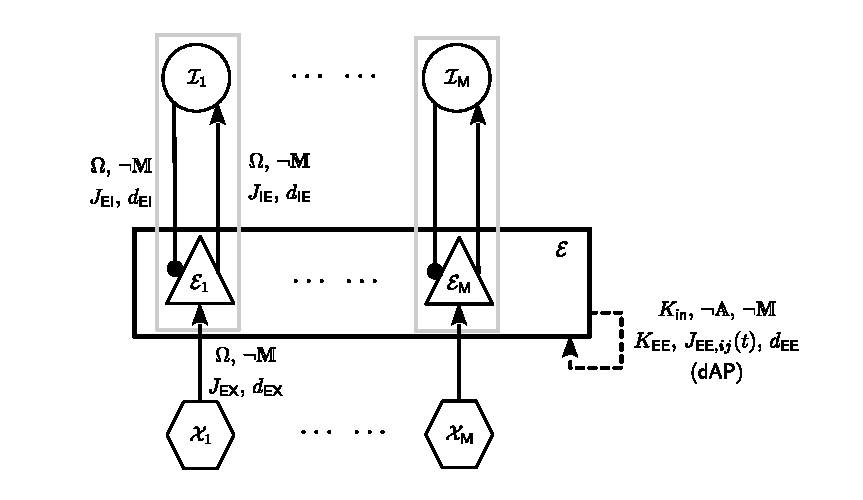
\includegraphics{figures/NetworkSketch_SpikingTemporalMemory.pdf}\\[-5ex] \hfill (see \href{https://doi.org/10.1371/journal.pcbi.1010086.g008}{legend})}}\\
\hline
\end{tabular}
%%%%%%%%%%%%%%%%%%%
\caption{Summary of the network model. Parameter values are given in Table \cref{tab:Model-parameters}.}
\label{tab:Model-description-summary}
\end{table}
%%%%%%%%%%%%%%%%%%%%%%%%%%%%%%%%%%%%%%%%%%%%%%%%%%%%%%%%%%%%%%%%%%%%%%%%%%%%%%%%%%%%
%% model description table (continued)
\begin{table}[H]
%%%%%%%%%%%%%%%%%%%
%%%%%%%%%%%%%%%%%%% 
\begin{tabular}{|@{\hspace*{1mm}}p{3cm}@{}|@{\hspace*{1mm}}p{10.95cm}@{}|@{\hspace*{1mm}}p{0.95cm}|}  
\hline 
\multicolumn{3}{|>{\color{white}\columncolor{black}}c|}{\textbf{Populations}}\\
\hline
$\Epop=\cup_{i=k}^M\mathcal{M}_k$ & excitatory (E) neurons  & $N_\exc$\\
  \hline
  $\Ipop$ & inhibitory (I) neurons & $N_\inh$\\
  \hline
  %$\Bpop=\cup_{i=k}^M\mathcal{Q}_k$ or $\mathcal{G}$ & background inputs & $M$\\
  %\hline
  $\mathcal{M}_k$ & excitatory neurons in subpopulation $k$, \mbox{$\mathcal{M}_k\cap\mathcal{M}_l=\emptyset\ (\forall{}k\ne{}l\in[1,M])$} & $n_\exc$ \\
  \hline
\end{tabular}
%%%%%%%%%%%%%%%%%%%
\caption{Description of the populations. Parameter values are given in \cref{tab:Model-parameters}}
\label{tab:Model-description-populations}
\end{table}

%%%%%%%%%%%%%%%%%%%%%%%%%%%
% CONNECTIVITY
%%%%%%%%%%%%%%%%%%%%%%%%%%%

\begin{table}[!ht]
  %\centering
  \renewcommand{\arraystretch}{1.2}
  \small
%%%%%%%%%%%%%%%%%%%
\begin{tabular}{|@{\hspace*{1mm}}p{1.85cm}@{}|@{\hspace*{1mm}}p{1.85cm}@{}|@{\hspace*{1mm}}p{11.2cm}|}
\hline 
\multicolumn{3}{|>{\color{white}\columncolor{black}}c|}{\textbf{Connectivity}}\\
\hline 
\textbf{Source population} & \textbf{Target population} & \textbf{Pattern}\\
\hline 
  $\Epop$  & $\Epop$ & random;
                       fixed in-degrees $K_i=K_\EE$, delays $d_{ij}=d_{\EE}$, and synaptic time constants $\tau_{ij}=\tau_{\EE}$,
                       plastic synaptic weights $J_{ij}$ 
                       ($\forall{}i\in{\Epop},\,\forall{}j\in{\Epop}$; ``$\EE$ connections'') \\
\hline 
  $\Epop$  & $\Ipop$ & all-to-all;
                       fixed delays $d_{ij}=d_{\IE}$, synaptic time constants $\tau_{ij}=\tau_{\IE}$, and weights $J_{ij}=J_\IE$
                       ($\forall{}i\in\mathcal\Ipop,\,\forall{}j\in{}\Epop$; ``$\IE$ connections'') \\
\hline 
  $\Ipop$ & $\Epop$ & all-to-all;
                      fixed delays $d_{ij}=d_{\EI}$, synaptic time constants $\tau_{ij}=\tau_{\EI}$, and weights $J_{ij}=J_\EI$
                      ($\forall{}i\in\Epop,\,\forall{}j\in{}\Ipop$; ``$\EI$ connections'') \\
\hline 
  $\Ipop$ & $\Ipop$ & none (``$\II$ connections'') \\
\hline
  all & all & no self-connections (``autapses''), no multiple connections (``multapses'') \\

\hline

\end{tabular}
%%%%%%%%%%%%%%%%%%%
\caption{Description of the connectivity. Parameter values are given in Table \cref{tab:Model-parameters}.}
\label{tab:Model-description-connectivity}
\end{table}
%%%%%%%%%%%%%%%%%%%%%%%%%%%%%%%%%%%%%%%%%%%%%%%%%%%%%%%%%%%%%%%%%%%%%%%%%%%%%%%%%%%%
%%%%%%%%%%%%%%%%%%%%%%%%%%%%%%%%%%%%%%%%%%%%%%%%%%%%%%%%%%%%%%%%%%%%%%%%%%%%%%%%%%%% 
\begin{table}[ht!]
%%%%%%%%%%%%%%%%%%%
\begin{tabular}{|@{\hspace*{1mm}}p{3cm}@{}|@{\hspace*{1mm}}p{12cm}|}
  \hline 
  \multicolumn{2}{|>{\color{white}\columncolor{black}}c|}{\textbf{Neuron}}\\
  %%%%%%%%%%%%%
  \hline
  \textbf{Type} & leaky integrate-and-fire (LIF) dynamics \\
  \hline
    \textbf{Description} & dynamics of membrane potential $V_{i}(t)$  and spiking activity $s_i(t)$ of neuron $i$:                
            \begin{itemize}
              \item emission of the $k$th spike of neuron $i$ at time $t_{i}^{k}$ if
                \begin{equation}
                  V_{i}(t_{i}^{k})\geq\theta_i %and $V_{i}\left(t_{k-1}^{i}\right)\leq\theta$
                \end{equation}
                 with somatic spike threshold $\theta_i$
              \item spike train: $s_i(t)=\sum_k\delta(t-t_i^k)$
              \item reset and refractoriness:
                \begin{equation*}
                  V_{i}(t)=\Vreset
                    \quad \forall{}k,\ \forall t \in \left(t_{i}^{k},\,t_{i}^{k}+\tau_{\text{ref},i}\right]
                \end{equation*}
                with refractory time $\tau_{\text{ref},i}$ and reset potential $\Vreset$
              \item subthreshold dynamics:
                \begin{equation}
                  \label{eq:lif}
                  \tau_{\text{m},i}\dot{V}_i(t)=-V_i(t)+R_{\text{m},i} I_i(t)
                \end{equation}
                with membrane resistance $R_{\text{m},i}=\dfrac{\tau_{\text{m},i}}{C_{\text{m},i}}$, membrane time constant $\tau_{\text{m},i}$, and total synaptic input current $I_i(t)$ (see \cref{tab:Model-description-synapse})
              \item excitatory neurons: $\tau_{\text{m},i}=\tau_\text{m,E}$, $C_{\text{m},i}=C_\text{m}$, $\theta_i=\theta_\text{E}$, $\tau_{\text{ref},i}=\tau_\text{ref,E}$ ($\forall i\in\Epop$)
              \item inhibitory neurons: $\tau_{\text{m},i}=\tau_{\text{m},I}$, $C_{\text{m},i}=C_\text{m}$, $\theta_i=\theta_\text{I}$, $\tau_{\text{ref},i}=\tau_\text{ref,I}$ ($\forall i\in\Ipop$)       
   
            \end{itemize}\\
              \hline 
\end{tabular}
%%%%%%%%%%%%%%%%%%%
\caption{Description of the neuron model. Parameter values are given in \cref{tab:Model-parameters}.}
\label{tab:Model-description-neuron}
\end{table}
%%%%%%%%%%%%%%%%%%%%%%%%%%%%%%%%%%%%%%%%%%%%%%%%%%%%%%%%%%%%%%%%%%%%%%%%%%%%%%%%%%%%

%%%%%%%%%%%%%%%%%%%%%%%%%%%%%%%%%%%%%%%
%%%% Synapse model
%%%%%%%%%%%%%%%%%%%%%%%%%%%%%%%%%%%%%%%

%%%%%%%%%%%%%%%%%%%%%%%%%%%%%%%%%%%%%%%
\begin{table}[ht!]
  %\begin{adjustwidth}{-.43in}{-.3in}   
  %\centering
  \small
  %%%%%%%%%%%%%
  \begin{tabular}{|@{\hspace*{1mm}}p{3cm}@{}|@{\hspace*{1mm}}p{12cm}|}
  %%%%%%%%%%%%%
  \hline
  \multicolumn{2}{|>{\color{white}\columncolor{black}}c|}{\textbf{Synapse}}\\
  \hline
  \textbf{Type} & continuous, exponential, or alpha-shaped postsynaptic currents (PSCs) \\
  \hline
  \textbf{Description} &                 
    \begin{itemize}
      \item  total synaptic input current
      \begin{equation}
        \label{eq:all_curr}
        \begin{aligned}
          \text{excitatory neurons:}\quad I_i(t) &= I_{\text{ED},i}(t) + I_{\text{EX},i}(t) + I_{\text{EI},i}(t) ,\ \forall i\in\Epop \\
          \text{inhibitory neurons:}\quad I_i(t) &= I_{\text{IE},i}(t) ,\ \forall i\in\Ipop
        \end{aligned}
      \end{equation}
      with dendritic, inhibitory, excitatory, and external input currents $I_{\text{ED},i}(t)$,  $I_{\text{EI},i}(t)$, $I_{\text{IE},i}(t)$, $I_{\text{EX},i}(t)$ evolving according to
      \begin{equation}
        \label{eq:dendritic_current}
          % \tau_\text{ED}\dot{I}_{\text{D},i} = -I_{\text{D},i}(t) + \sum_{j\in\Epop} \alpha(t) s_j(t-d_{ij})
          I_{\text{ED},i}(t)=\sum_{j\in\Epop}(\alpha_{ij}*s_j)(t-d_{ij})
    \end{equation}
    \qquad with $\alpha_{ij}(t)=J_{ij} \dfrac{e}{\tau_{\text{ED}}} t e^{-t/\tau_{\text{ED}}} \Theta(t)$
    and
    $
    \Theta(t)=
    \begin{cases}1 & t \ge 0 \\ 0 & \text{else} \end{cases}
    $
    \begin{equation}
      \label{eq:EI_current}
      \tau_\text{EI}\dot{I}_{\text{EI},i} = -I_{\text{EI},i}(t) + \sum_{j\in\Ipop} J_{ij} s_j(t-d_{ij})
    \end{equation}
    \begin{equation}
      \label{eq:IE_current}
      \tau_\text{IE}\dot{I}_{\text{IE},i} = -I_{\text{IE},i}(t) + \sum_{j\in\Epop} J_{ij} s_j(t-d_{ij})
    \end{equation}
    \begin{equation}
      \label{eq:EX_current}
      %\tau_\text{EX}\dot{I}_{\text{EX},i} = -I_{\text{EX},i}(t) + \sum_{j\in\Xpop} J_{ij} s_j(t-d_{ij})
      I_{\text{EX},i}(t)=I_{\text{S},i}(t)+I_{\text{B},i}(t)
    \end{equation}
    where $I_{\text{S},i}(t)$ is the stimulus input (see \cref{tab:Model-description-inout}:Input).
    \item suprathreshold dynamics of dendritic currents (dAP generation):
      \begin{itemize}
      \item emission of $k$th dAP of neuron $i$ at time $t_{\text{dAP},i}^k$ if $ I_{\text{ED},i}(t_{\text{dAP},i}^k)\geq\theta_{\text{dAP}}$
      \item dAP current plateau:
      \begin{equation}
        \label{eq:dAP_current_nonlinearity}
        I_{\text{ED},i}(t) = I_\text{dAP}
        \quad\forall{}k,\ \forall t \in \left(t_{\text{dAP},i}^k,t_{\text{dAP},i}^k+\tau_\text{dAP}\right)
      \end{equation}
      with
      dAP current plateau amplitude $I_\text{dAP}$,
      dAP current duration $\tau_\text{dAP}$, and
      dAP activation threshold $\theta_{\text{dAP}}$
      \item reset: $I_{\text{ED},i}(t_{\text{dAP},i}^k+\tau_\text{dAP})=0$ ($\forall{}k$)
      \item reset and refractoriness in response to emission of $l$th somatic spike of neuron $i$ at time $t_{i}^{l}$:
      \begin{equation}
        I_{\text{ED},i}(t)=0
        \quad \forall{}l,\ \forall t \in \left(t_{i}^{l},\,t_{i}^{l}+\tau_{\text{ref},i}\right)
      \end{equation}
      \item[]
    \end{itemize}
    \end{itemize} \\
   \hline 
\end{tabular}
%%%%%%%%%%%%%%%%%%%
%%%%%%%%%%%%%%%%%%%
\caption{Description of the synapse model. Parameter values are given in \cref{tab:Model-parameters}.}
\label{tab:Model-description-synapse}
%\end{adjustwidth}
\end{table}

%%%%%%%%%%%%%%%%%%%%%%%%%%%%%%%%%%%%
%%% Plasticity
%%%%%%%%%%%%%%%%%%%%%%%%%%%%%%%%%%%%%
%\setcounter{table}{\thetable-1}
\begin{table}[ht!]
%  \begin{adjustwidth}{-.43in}{-.3in} 
  %\centering
  \small
  %%%%%%%%%%%%%%%%%%%
  \begin{tabular}{|@{\hspace*{1mm}}p{3cm}@{}|@{\hspace*{1mm}}p{12.cm}|}
  \hline 
  \multicolumn{2}{|>{\color{white}\columncolor{black}}c|}{\textbf{Plasticity}}\\
  \hline
  \textbf{Type} & spike-timing dependent structural plasticity and permanence decay \\
  \hline
  \textbf{EE synapses} &
      \begin{itemize}  
        \item dynamics of synaptic permanence $P_{ij}(t)$ (maturity) in EE connections during learning:
          \begin{equation}
            \label{eq:plasticity}
          % \begin{aligned}
          %   &\forall J_\text{min}<J_{ij}<J_\text{max}: \\[1ex]
          %   & \quad J_\text{max}^{-1}\frac{dJ_{ij}}{dt} = \lambda_{+} \sum_{\{t_i^*\}^\prime} x_j(t) \delta(t-[t_i^*+d_\EE]) I(t_i^*,\Delta{}t_\text{min},\Delta{}t_\text{max}) \\
          %   & - \lambda_{-} y_i \sum_{\{t_j^*\}} \delta(t-t_j^*) \\
          %   & + \lambda_\text{h}  \sum_{\{t_i^*\}^\prime} \bigl( z^* - z_i(t) \bigr) \delta(t-t_i^*)I(t_i^*,\Delta{}t_\text{min},\Delta{}t_\text{max}).\\
          %   & \forall{}\{t|J_{ij}(t)<J_\text{min}\}: \quad J_{ij}(t)=J_\text{min}\\
          %   &\forall{}\{t|J_{ij}(t)>J_\text{max}\}: \quad J_{ij}(t)=J_\text{max}
          % \end{aligned}  
          \begin{aligned}
            \forall P_\text{min}<P_{ij}<P_\text{max}&: \\[1ex]
            \frac{dP_{ij}}{dt} &= P_\text{max} \, \lambda_{+} \sum_{\{t_i^*\}^\prime} \delta(t-[t_i^*+d_\EE]) I_{+}(x_j(t), t_i^*,\Delta{}t_\text{min},\Delta{}t_\text{max}) \\
            &\quad - P_\text{max} \, \lambda_{-} \sum_{\{t_j^*\}^\prime} \delta(t-[t_j^*+d_\EE]) I_{-}(x_i(t),t_j^*,\Delta{}t_\text{max}) \\
            &\quad + (P_\text{min}-P) \frac{1}{\tau_\text{P}}\\
            & \forall{}\{t|P_{ij}(t)<P_\text{min}\}: \quad P_{ij}(t)=P_\text{min}\\
            &\forall{}\{t|P_{ij}(t)>P_\text{max}\}: \quad P_{ij}(t)=P_\text{max}
          \end{aligned}  
        \end{equation}
        with
        \begin{itemize}
        \item list of presynaptic spike times $\{t_j^*\}$,
        \item list of postsynaptic spike times %\newline
          \mbox{$\{t_i^*\}^\prime=\{t_i^*| \forall{}t_j^*:\,t_i^*-t_j^*+d_\EE\ge\Delta{}t_\text{min}\}$}  
        \item increment functions
          \begin{equation}
            \label{eq:indicator_function}
            \begin{aligned}
              I_{+}(x_j(t),t_i^*,\Delta{}t_\text{min},\Delta{}t_\text{max})&=R_{+}(t_i^*-t_j^{+}+d_\EE)\\
              \text{with}\quad
              R_{+}(\tau)&=\
              \begin{cases}
                x_j(t) & \Delta{}t_\text{min}<\tau<\Delta{}t_\text{max}\\
                (x_j(t)-1) & \tau<\Delta{}t_\text{min}\\
                0 & \text{else},
              \end{cases}\\
              I_{-}(x_i(t),t_j^*,\Delta{}t_\text{max})&=R_{-}(t_j^*-t_i^{-}+d_\EE)\\
              \text{with}\quad
              R_{-}(\tau)&=\
              \begin{cases}
                x_i(t) & \tau<\Delta{}t_\text{max}\\
                0 & \text{else},
              \end{cases}
            \end{aligned}
          \end{equation}
        \item maximum permanence $P_\text{max}$, minimum permanence $P_\text{max}$, potentiation and depression rates $\lambda_\text{+}$, $\lambda_\text{-}$, decay time constant $\tau_\text{P}$, delay $d_\EE$, minimum $\Delta{}t_\text{min}$ and maximum $\Delta{}t_\text{max}$ time lags between pairs of pre- and postsynaptic spikes at which synapses are potentiated or depressed, nearest presynaptic spike time $t_j^{+}$ preceding $t_i^*$, nearest postsynaptic spike time $t_i^{-}$ preceding $t_j^*$,
        \item spike trace of presynaptic neuron $j$, evolving according to
        \begin{equation*}
          \frac{dx_j}{dt}=-\tau_{+}^{-1} x_j(t) + \sum_{t_j^*}\delta(t-t_j^*)
        \end{equation*}
        with presynaptic spike times $t_j^*$ and potentiation time constant $\tau_{+}$,
        \item spike trace of postynaptic neuron $i$, evolving according to
        \begin{equation*}
          \frac{dx_i}{dt}=-\tau_{-}^{-1} x_i(t) + \sum_{t_i^*}\delta(t-t_i^*)
        \end{equation*}
        with postynaptic spike times $t_i^*$ and depression time constant $\tau_{-}$.
        \end{itemize}
        %% TODO: How do I bring in tau_{-} here? tau_{-} is the time constant of the presynaptic neuron j ?stdp
        %%
        \item dynamics of synaptic weights $J_{\EE, ij}$ according to
        \begin{equation*}
            J_{\EE, ij} = \begin{cases}J_\mathrm{max} & P_{ij} > P_\theta \\ 0 & \text{else}, \end{cases}
        \end{equation*}
        with maximum synaptic weight $J_\text{max}$ and synapse maturity threshold $P_\theta$.
      \end{itemize}\\ 
  \hline 
  \textbf{all other synapses} & non-plastic
  \\
  \hline
\end{tabular}
%%%%%%%%%%%%%%%%%%%
\caption{Description of the plasticity model. Parameter values are given in \cref{tab:Model-parameters}.}
\label{tab:Model-description-plasticity}
%\end{adjustwidth}
\end{table}


%%%%%%%%%%%%%%%%%%%%%%%%%%%%%%%%%%%%%%%%%%%%%%%%%%%%%%%%%%%%%%%%%%%%%%%%
%%%%%%%%%%%%%%%%%%%
\begin{table}
\begin{tabular}{|@{\hspace*{1mm}}p{15.15cm}|}
%\hline 
  \multicolumn{1}{|>{\color{white}\columncolor{black}}c|}{\textbf{Input}}\\
  %\begin{itemize}
  %\item $N_\text{stim}$ spike-generating sources, each representing a character in the sequences
  %\item each spike source connected to a random subset of $L$ subpopulations via a synaptic weight $J_\EF$ and a delay of $d_\EF$
  %\end{itemize}
    \begin{itemize}
      \item repetitive stimulation of the network using the same
        set $\mathcal{S}=\{s_1,\ldots,s_{S}\}$ of
        sequences $s_i=$\seq{$\zeta_{i,1}$, $\zeta_{i,2}$,\ldots, $\zeta_{i,C_i}$} of
        ordered discrete items $\zeta_{i,j}$ 
        with number of sequences $S$ and length $C_i$ of $i$th sequence
        \item presentation of sequence element $\zeta_{i,j}$ at time $t_{i,j}$ modeled by a single spike $x_k(t)=\delta(t-t_{i,j})$ generated by the corresponding external source $x_k$
        \item generated current as a response to the presentation of the sequence elements:
        \begin{equation}
          \tau_\text{S}\dot{I}_{\text{S},i} = -I_{\text{S},i}(t) + \sum_{j \in \mathcal{X}} J_{i,j} x_j(t-d_{ij})        
        \end{equation} 
    
        \item inter-stimulus interval $\Delta{}T=t_{i,j+1}-t_{i,j}$ between subsequent sequence elements $\zeta_{i,j}$ and $\zeta_{i,j+1}$ within a sequence $s_i$
        \item inter-sequence time interval $\Delta{}T_\text{seq}=t_{i+1,1}-t_{i,C_i}$ between subsequent sequences $s_i$ and $s_{i+1}$
        \item example sequence sets: 
          \begin{itemize}
          \item sequence set I: $\mathcal{S}$=\{\seq{A,F,B,D}, \seq{A,F,C,E}\}
          \item sequence set II: $\mathcal{S}$=\{\seq{A,F,B,D}, \seq{A,F,C,E}, \seq{A,F,G,H}, \seq{A,F,I,J}, \seq{A,F,K,L}\}
          \end{itemize} 
        \item sequence $i$ of length $C_i$ is generated by uniformly and independently drawing $C_i$ elements from a vocabulary of $A$ unique token with equal probability
    \end{itemize}
  \\
\hline 
\multicolumn{1}{|>{\color{white}\columncolor{black}}c|}{\textbf{Output}} \\
  \hline
    \begin{itemize}
    \item somatic spike times $\{t_i^k | \forall{}i\in\mathcal{E},k=1,2,\ldots \}$
    \item dendritic currents $I_{\text{ED},i}(t)$ ($\forall{}i\in\mathcal{E}$)
    \end{itemize} \\
  \hline
\end{tabular}
%%%%%%%%%%%%%%%%%%%
  \caption{Description of the input and the output. Parameter values are given in \cref{tab:Model-parameters}.}
  \label{tab:Model-description-inout}
\end{table}

%%%%%%%%%%%%%%%%%%%%%%%%
%%% INITIAL CONDITIONS &  SIMULATION DETAILS
%%%%%%%%%%%%%%%%%%%%%%%%
\begin{table}
\begin{tabular}{|@{\hspace*{1mm}}p{15.15cm}|}
  \multicolumn{1}{|>{\color{white}\columncolor{black}}c|}{\textbf{Initial conditions and network realizations}} \\
    \begin{itemize}
    \item membrane potentials: $V_i(0)=V_\text{r}$ ($\forall{}i\in\mathcal{E}\cup\mathcal{I}$)
    \item dendritic currents: $I_{\text{ED},i}(0)=0$ ($\forall{}i\in\mathcal{E}$)
    \item external currents: $I_{\text{EX}}(0)=0$ ($\forall{}i\in\mathcal{E}$)
    \item inhibitory currents: $I_{\text{EI},i}(0)=0$ ($\forall{}i\in\mathcal{E}$)
    \item excitatory currents: $I_{\text{IE},i}(0)=0$ ($\forall{}i\in\mathcal{I}$)
    \item synaptic permanences: $P_{ij}(0)\sim\mathcal{U}(P_{0,\text{min}},P_{0,\text{max}})$ (uniform distribution; $\forall{}i,j\in\mathcal{E}$)
    \item synaptic weights: $\J_{ij}(0)=0$ ($\forall{}i,j\in\mathcal{E}$)
    \item spike traces: $x_i(0)=0$ ($\forall{}i\in\mathcal{E}$)
    \item connectivity and initial weights are randomly and independently drawn for each network realization
    \end{itemize}\\
    \hline
  \end{tabular}
%%%%%%%%%%%%%%%%%%%
 \begin{tabular}{|@{\hspace*{1mm}}p{15.15cm}|}
  \multicolumn{1}{|>{\color{white}\columncolor{black}}c|}{\textbf{Simulation details}}\\
  \hline
  \begin{itemize}
  \item network simulations performed in NEST \citep{Gewaltig_07_11204} version 3.6 \citep{Nest360}.
  \item definition of excitatory neuron model and plastic synapse model using NESTML \citep{Plotnikov16_93,Linssen25_1544143} version 8.0.0 \citep{Linssen24_nestml8.0.0}.
  \item synchronous update using exact integration of system dynamics on discrete-time grid with step size $\dtsim$ \cite{Rotter99a}
  %\item source code underlying this study: %\url{https://doi.org/10.5281/zenodo.6378376}
  \end{itemize}
  \\
  \hline
\end{tabular}
%%%%%%%%%%%%%%%%%%%
\caption{Description of the initial conditions and simulation details. Parameter values are given in \cref{tab:Model-parameters}.}
\label{tab:Model-description-initcond}
\end{table}

\clearpage

\subsection{Model and simulation parameters}
\label{app:suppl_parameters}

%%%%%%%%%%%%%%%%%%%%%%%%%%%%%%%%%%%%%%%%%%%%%%%%%%%%%%%%%%%%%%%%%%%%%%%%%%%%%%%%%%%%
\begin{table}[ht!]
\renewcommand{\arraystretch}{1.2}
\begin{tabular}{|@{\hspace*{1mm}}p{3cm}@{}|@{\hspace*{1mm}}p{4cm}@{}|@{\hspace*{1mm}}p{8.1cm}|}
\hline
\textbf{Name} & \textbf{Value} & \textbf{Description}\\
\hline                               
\multicolumn{3}{|>{\columncolor{lightgray}}c|}{\textbf{Network}}\\
%\hline 
%\textbf{Name} & \textbf{Value} & \textbf{Description}\\
\hline 
$N_\exc$ & $6240$ & number of excitatory neurons \\
\hline
$N_\inh$ & $26$ & number of inhibitory neurons \\
\hline
$M$ & $26$ & number of subpopulations \\
\hline
$\nE$,$\nI$ & $240$,$1$ & number of excitatory and inhibitory neurons per subpopulation \\
\hline
$\rho$ & $20$ & (target) number of active neurons per subpopulation after learning = minimal number of coincident excitatory inputs required to trigger a spike in postsynaptic inhibitory neurons \\
\hline 
$N_\text{X}$ & $26$ & number of external spike sources \\
\hline
\multicolumn{3}{|>{\columncolor{lightgray}}c|}{\textbf{(Potential) Connectivity}}\\
%\hline 
%\textbf{Name} & \textbf{Value } & \textbf{Description}\\
\hline
$\KEE$ & $936$ & number of excitatory inputs per excitatory neuron ($\EE$ in-degree) \\
\hline 
$p$ & $K_{\exc\exc}/N_\exc=0.15$ & connection probability \\
\hline 
$\KEI$ & $1$ & number of inhibitory inputs per excitatory neuron ($\EI$ in-degree) \\
\hline 
$\KIE$ & $\nE$ & number of excitatory inputs per inhibitory neuron ($\IE$ in-degree) \\
\hline 
$\KII$ & $0$ & number of inhibitory inputs per inhibitory neuron ($\II$ in-degree) \\
%\hline 
%\end{tabular}
%%%%%%%%%%%%%%%%%%%%%%%%%%%%%%%%%%%%%%%%%%%%%
%\begin{tabular}{|@{\hspace*{1mm}}p{3cm}@{}|@{\hspace*{1mm}}p{4cm}@{}|@{\hspace*{1mm}}p{8.1cm}|}
\hline 
\multicolumn{3}{|>{\columncolor{lightgray}}c|}{\textbf{Excitatory neurons}}\\
\hline 
$\tau_\text{m,E}$ & $10\ms$ & membrane time constant \\
\hline 
$\tau_\text{ref,E}$ & $10\ms$ & absolute refractory period \\
\hline 
$\CM$ & $250\pF$ & membrane capacity \\
\hline 
$\Vreset$ & $0.0\mV$ & reset potential \\
\hline 
$\theta_\text{E}$ & $20\mV$ & somatic spike threshold \\
\hline 
$I_\text{dAP}$ & $200\pA$ &  dAP current plateau amplitude\\
\hline 
$\tau_\text{dAP}$ & $60\ms$ & dAP duration\\
\hline 
$\theta_{\text{dAP}}$ & $59\pA$ & dAP threshold \\
%\hline
%\end{tabular}
%\begin{tabular}{|@{\hspace*{1mm}}p{3cm}@{}|@{\hspace*{1mm}}p{4cm}@{}|@{\hspace*{1mm}}p{8.1cm}|}
%%%%%%%%%%%%%%%%%%%%%%%%%%%%%%%%%%%%%%%%%%%%%
\hline 
\multicolumn{3}{|>{\columncolor{lightgray}}c|}{\textbf{Inhibitory neurons}}\\
\hline
$\tau_\text{m,I}$ & $5\ms$ & membrane time constant\\
\hline 
$\tau_\text{ref,I}$ & $2\ms$ & absolute refractory period\\
\hline 
$\CM$ & $250\pF$ & membrane capacity\\
\hline 
$\Vreset$ & $0.0\mV$ & reset potential\\
\hline 
$\theta_\text{I}$ & $15\mV$ & spike threshold\\
\hline
\end{tabular}
%%%%%%%%%%%%%%%%%%%
\caption{Model and simulation parameters (continued on next page).}
\label{tab:Model-parameters} 
\end{table}
%%%%%%%%%%%%%%%%%%%%%%%%%%%%%%%%%%%%%%%%%%%%%%%%%%%%%%%%%%%%%%%%%%%%%%%%%%%%%%%%%%%%
%%%%%%%%%%%%%%%%%%%%%%%%%%%%%%%%%%%%%%%%%%%%%%%%%%%%%%%%%%%%%%%%%%%%%%%%%%%%%%%%%%%% 
\setcounter{table}{\thetable-1}
\begin{table}[ht!]
%%%%%%%%%%%%%%%%%%%
\begin{tabular}{|@{\hspace*{1mm}}p{3cm}@{}|@{\hspace*{1mm}}p{4cm}@{}|@{\hspace*{1mm}}p{8.1cm}|}
\hline
\textbf{Name} & \textbf{Value } & \textbf{Description}\\
\hline
\multicolumn{3}{|>{\columncolor{lightgray}}c|}{\textbf{Synapse}}\\
%\hline 
%\textbf{Name} & \textbf{Value } & \textbf{Description}\\
\hline
$\JIE$ & $\sim{}581.19\pA$ & weight of IE connections (EPSC amplitude) \\
\hline
%$\tilde{J}_\text{EI}$ & $-40 \mV$ & weight of EI connections (IPSP amplitude) \\
%\hline 
$\JEI$ & $\sim{}-12915.49\pA$ & weight of EI connections (IPSC amplitude) \\
\hline 
%$\tilde{J}_\text{EX}$ & $22 \mV$ & weight of EX connections (EPSP amplitude) \\
%\hline 
$\JEX$ & $\sim{}4112.20\pA$ & weight of EX connections (EPSC amplitude) \\
\hline
${\tau}_{\EE}$ & $5\ms$ & synaptic time constant of EE connections\\
\hline 
${\tau}_{\EI}$ & $1\ms$ & synaptic time constant of EI connections\\
\hline 
${\tau}_{\EX}$ & $2\ms$ & synaptic time constant of EX connection\\
\hline 
${\tau}_{\IE}$ & $0.5\ms$ & synaptic time constant of IE connections\\
\hline
$d_{\EE}$ & $2\ms$ & delay of EE connections (dendritic)\\
\hline
$d_\IE$ & $0.1\ms$ & delay of IE connections\\
\hline
$d_\EI$ & $0.1\ms$ & delay of EI connections\\
\hline 
$d_\EX$ & $0.1\ms$ & delay of EX connections\\
\hline 
\multicolumn{3}{|>{\columncolor{lightgray}}c|}{\textbf{Plasticity}}\\
\hline
$\lambda_{+}$ & $0.6$  & potentiation rate \\
\hline
$\lambda_{-}$ & $\{0.1, 0.8\}$ & depression rate \\
\hline
$P_{ij}$ & $[P_\text{min},P_0]$  & synaptic permanence \\
\hline
$P_{\theta}$ & 20 & synapse maturity threshold
% when the permanence reaches this value the plastic weight ($\JEE$) becomes W
                            \\
\hline
$P_\text{max}$ & 20 & permanence upper bound\\
\hline
$P_\text{min}$ & 1 & permanence lower bound  \\
\hline
$P_{0,\mathrm{max}}$ & 8 & permanence initialization upper bound \\
\hline
$P_{0,\mathrm{min}}$ & 0 & permanence initialization upper bound \\
\hline         
$J_\text{max}$ & $12.98\pA$ & maximum weight\\
\hline
$ \tau_{+} $ & 20 \ms & plasticity time constant (potentiation) \\
\hline
$ \tau_{-} $ & 20 \ms & plasticity time constant (depression) \\
\hline                        
$ \tau_{\mathrm{P}} $ & $80\s$ & permanence leak time constant \\
\hline
$\Delta{}t_\text{min}$ & $4\ms$ & minimum time lag between pairs of pre- and postsynaptic spikes at which synapses are potentiated given the spike trace of the presynaptic neuron of the current time step \\ %TODO: find a better description here
\hline
$\Delta{}t_\text{max}$ & $50\ms$ & maximum time lag between pairs of pre- and postsynaptic spikes at which synapses are potentiated \\
\hline                                             
\multicolumn{3}{|>{\columncolor{lightgray}}c|}{\textbf{Input}}\\
%\hline 
%\textbf{Name} & \textbf{Value } & \textbf{Description}\\
\hline 
%$L$ & $1$ & number of subpopulations connected to the same spike source \\
%\hline
$S$ & 1 & number of sequences per sequence set \\
\hline
$C_i$ & $[10, 150]$ & number of characters per sequence \\
\hline
$A$ & 26 & alphabet length \\
%\hline 
%\end{tabular}
%%%%%%%%%%%%%%%%%%%%%%%%%%%%%%%%%%%%%%%%%%%%%
%\begin{tabular}{|@{\hspace*{1mm}}p{3cm}@{}|@{\hspace*{1mm}}p{4cm}@{}|@{\hspace*{1mm}}p{8.1cm}|}
\hline 
$\Delta{}T$ & $50\ms$ & inter-stimulus interval (during training)\\
\hline
%$N_\text{t}$ & $[??, ??]$ & number of cue presentations (trials) \\
%\hline
%$\Delta{}T_\text{cue}$ & $100\ms$ & inter-cue interval \\
%\hline
$\Delta{}T_\text{seq}$ & $\mathcal{U}(100, 105)\ms$ $\qquad \quad$ (uniform distribution) & inter-sequence interval \\
\hline
\multicolumn{3}{|>{\columncolor{lightgray}}c|}{\textbf{Simulation}}\\
%\hline 
%\textbf{Name} & \textbf{Value } & \textbf{Description}\\
\hline
$\dtsim$ & $0.1\ms$ & time resolution \\
\hline
\end{tabular}
%%%%%%%%%%%%%%%%%%%%%%%%%%%%%%%%%%%%%%%%%%%%%
\caption{Model and simulation parameters.}
\label{tab:Model-parameters} 
\end{table}

\newpage

%%%%%%%%%%%%%%%%%%%%%%%%%%%%%%%%%%%%%%%%%%%%%%%%%%%%%%%%%%%%%%%%%%%%
% add bibliography 
\begin{thebibliography}{}

\bibitem[\protect\citeauthoryear{Gewaltig \& Diesmann}{2007}]{Gewaltig_07_11204}
{Gewaltig, Marc-Oliver and Diesmann, Markus}
Gewaltig, M.-O., \& Diesmann, M. (2007).
\newblock {NEST} ({NE}ural {S}imulation {T}ool).
\newblock ScholarpediaJ, 4, 1430, https://doi.org/10.4249/scholarpedia.1430

\bibitem[\protect\citeauthoryear{Villamar et~al.}{Villamar
  et~al.}{2023}]{Nest360}
Villamar, J., Vogelsang, J., Linssen, C., Kunkel, S., Kurth, A., Sch\"{o}fmann, C.~M., Benelhedi, M.~A., Babu, P.~N., Eppler, J.~M., de Schepper, R., Mitchell, J., Morrison, A., Haug, N., Diaz, S., Acimovic, J., Graber, S., Jiang, H.-J., Terhorst, D., Spreizer, S., Welle Skaar, J.-E., Stapmanns, J., Manninen, T., Krüger, M., Lehtimäki, M., Ito, S., Lee, A. Y., Lindahl, M. \& Plesser, H.~E.
\newblock NEST 3.6

\bibitem[\protect\citeauthoryear{Plotnikov et~al.}{2016}]{Plotnikov16_93}
Plotnikov, D., Blundell, I., Ippen, T., Eppler, J.~M., Rumpe, B., Morrison, A.
\newblock {NESTML}: a modeling language for spiking neurons.
\newblock Modellierung 2016, P-254, pages 93-108

\bibitem[\protect\citeauthoryear{Linssen et~al.}{2025}]{Linssen25_1544143}
Linssen, C., Babu, P.~N., Eppler, J.~M., Koll, L., Rumpe, B., Morrison, A.
\newblock {NESTML}: a generic modeling language and code generation tool for the simulation of spiking neural networks with advanced plasticity rules.
\newblock Frontiers Neuroinformatics, 19, 10.3389/fninf.2025.1544143

\bibitem[\protect\citeauthoryear{Linssen et~al.}{2024}]{Linssen24_nestml8.0.0}
Linssen, C., Bouhadjar, Y., Ewert, L., Lober, M.,  Babu, P., Feller, F., Wybo, W., Morrison, A., Rumpe, B.
\newblock {NESTML} (v8. 0.0)

\bibitem[\protect\citeauthoryear{Rotter \& Diesmann}{Rotter \&
  Diesmann}{1999}]{Rotter99a}
Rotter, S., \& Diesmann, M. (1999).
\newblock Exact digital simulation of time-invariant linear systems with
  applications to neuronal modeling.
\newblock {\em Biol. Cybern.\/}~{\em 81\/}(5-6), 381--402.

\end{thebibliography}

\end{document}

%%% Local Variables:
%%% mode: latex
%%% TeX-master: t
%%% End:


\end{document}
